\documentclass[tikz,border=8pt]{standalone}
\usepackage{amsmath}
\usetikzlibrary{arrows.meta,positioning,fit}

\begin{document}
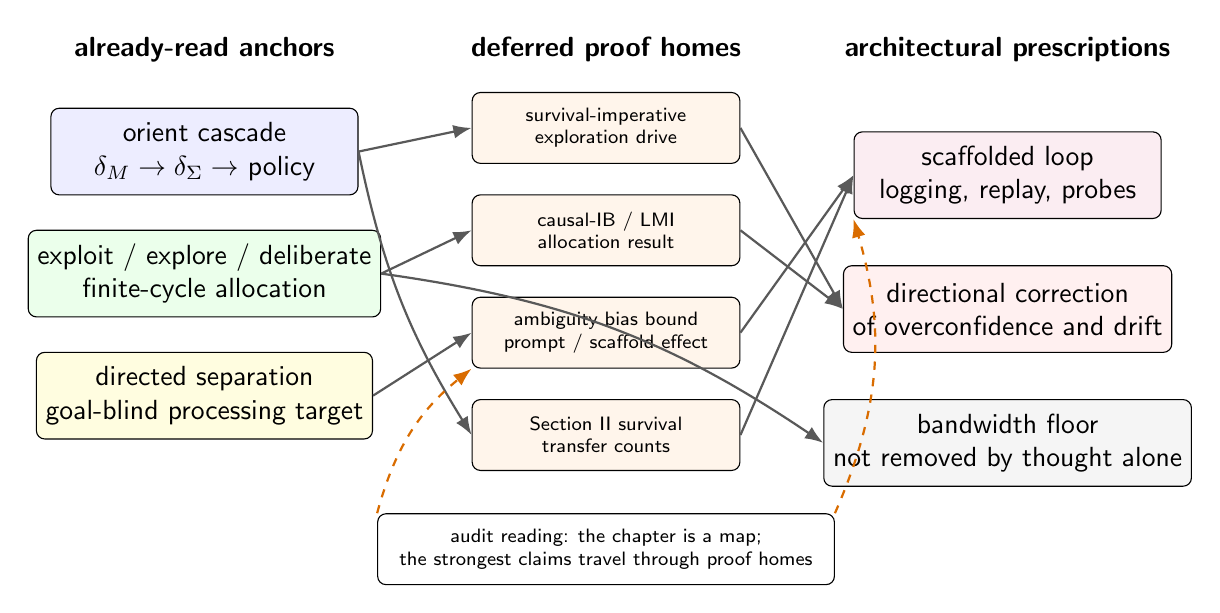
\begin{tikzpicture}[
  font=\sffamily,
  box/.style={draw, rounded corners=3pt, align=center, minimum width=39mm, minimum height=11mm, fill=white},
  small/.style={draw, rounded corners=3pt, align=center, font=\sffamily\scriptsize, minimum width=34mm, minimum height=9mm, fill=white},
  title/.style={align=center, font=\sffamily\bfseries},
  arrow/.style={-Latex, thick, draw=black!65},
  dashedarrow/.style={-Latex, thick, dashed, draw=orange!85!black}
]

\node[title] at (0,3.3) {already-read anchors};
\node[title] at (5.1,3.3) {deferred proof homes};
\node[title] at (10.2,3.3) {architectural prescriptions};

\node[box, fill=blue!7] (cascade) at (0,2)
  {orient cascade\\$\delta_M \to \delta_\Sigma \to$ policy};
\node[box, fill=green!8] (three) at (0,0.45)
  {exploit / explore / deliberate\\finite-cycle allocation};
\node[box, fill=yellow!12] (sep) at (0,-1.1)
  {directed separation\\goal-blind processing target};

\node[small, fill=orange!8] (surv) at (5.1,2.3)
  {survival-imperative\\exploration drive};
\node[small, fill=orange!8] (lmi) at (5.1,1.0)
  {causal-IB / LMI\\allocation result};
\node[small, fill=orange!8] (bias) at (5.1,-0.3)
  {ambiguity bias bound\\prompt / scaffold effect};
\node[small, fill=orange!8] (counts) at (5.1,-1.6)
  {Section II survival\\transfer counts};

\node[box, fill=purple!7] (scaffold) at (10.2,1.7)
  {scaffolded loop\\logging, replay, probes};
\node[box, fill=red!6] (direction) at (10.2,0)
  {directional correction\\of overconfidence and drift};
\node[box, fill=gray!8] (floor) at (10.2,-1.7)
  {bandwidth floor\\not removed by thought alone};

\draw[arrow] (cascade.east) -- (surv.west);
\draw[arrow] (three.east) -- (lmi.west);
\draw[arrow] (sep.east) -- (bias.west);
\draw[arrow] (cascade.east) to[bend right=10] (counts.west);

\draw[arrow] (surv.east) -- (direction.west);
\draw[arrow] (lmi.east) -- (direction.west);
\draw[arrow] (bias.east) -- (scaffold.west);
\draw[arrow] (counts.east) -- (scaffold.west);
\draw[arrow] (three.east) to[bend left=13] (floor.west);

\node[small, fill=white, minimum width=58mm] (caveat) at (5.1,-3.05)
  {audit reading: the chapter is a map;\\the strongest claims travel through proof homes};
\draw[dashedarrow] (caveat.north west) to[bend left=18] (bias.south west);
\draw[dashedarrow] (caveat.north east) to[bend right=20] (scaffold.south west);

\end{tikzpicture}
\end{document}
